\documentclass[dissertation.tex]{subfiles}

%TC:group code 0 0
%TC:group figure 0 0
%TC:macrocount \UoC 4
%TC:macrocount \mifare 1
%TC: macrocount \crypto 1
% chktex-file 29 (suppress "times might look prettier warning")

\begin{document}
  \chapter{Implementation}

  In this chapter, I explain how I implemented my project, justifying decisions made and describing the difficulties I faced. Explanations of \mifare{} concepts not previously introduced are included where appropriate. The implementation consists of the following:
  \begin{itemize}
    \item A library for interacting with, and simulating \mifare{} cards
    \item A library for reading and writing signed data to \mifare{} cards
    \item A simulation suite for simulating large networks of readers and cards
    \item A gossip protocol for distributing revoked UIDs to offline readers
  \end{itemize}

  \section{\mifare{} Library Implementation}

  The \mifare{} library is a library written in Go, upon which the rest of my implementation sits. It provides an API for interacting with \mifare{} cards and a software implementation of the card to support unit tests and simulations.

  \subsection{Structure of Library}
  The library is split into two parts, interfaces and drivers\footnote{I didn't use the more suitable object-oriented term ``implementations'' to prevent it from becoming overloaded within this chapter.}. The interfaces specify the publicly exposed objects the library provides and their public method signatures. The drivers are specific implementations that satisfy these interfaces.

  By splitting the library in this way, the public API exposed by the library is abstracted from the implementation. This means that any code built on top of the interfaces exposed by the library will work with any driver (implementation) that satisfies the interfaces. This flexibility has many benefits, including:

  \begin{itemize}
    \item \bold{Support mock drivers} \\
      Code that uses the library can be easily tested using a mock driver. The mock driver provides an in-memory implementation of readers and cards that satisfy the exported interfaces. Without this, any unit test would be dependent on physical hardware --- making it more fragile and harder to run regularly.

    \item \bold{Support platforms without libnfc} \\
      The library contains a driver (implementation) that uses libnfc and a mock one as this was required for my project. It would, however, be possible to write a driver that does not depend on libnfc. This would be useful on platforms such as Android where a system API is provided and libnfc may not be supported due to security sandboxing restrictions.
  \end{itemize}

  \subsection{Exported Interfaces and Types}
  The public API consists of a series of interfaces and types. In this section I explain them by including their definitions and providing background explanation where appropriate.

  \subsubsection{Driver and Device}
  The \texttt{Driver} is the base interface that has a method for listing available NFC readers and connecting to them.

  \begin{code}[numbers=none]{Go}
    type Driver interface {
    	// Name returns a string name for this driver e.g "libfreefare wrapper". It is
    	// typically only used in debug output.
    	Name() string

    	// ListDevices returns a list of connection strings or an error.
    	ListDevices() ([]string, error)

    	// Open takes a connection string and returns the Device corresponding to it
    	// or an error. If conn is empty then it connects to the first available device.
    	Open(conn string) (Device, error)
    }
  \end{code}

  A \texttt{Device} represents a connected NFC reader. It supports listing tags (cards) within the reader's field and closing the connection to the reader.

  \begin{code}[numbers=none]{Go}
    // Device represents an NFC device (e.g. USB reader)
    type Device interface {
    	// ListTags returns a list of Tags (cards) that are currently within the
    	// reader's field
    	ListTags() ([]Tag, error)

    	// Close closes the connection to the device
    	Close() error
    }
  \end{code}

  \subsubsection{Tag and TagType}
  The \texttt{Tag} interface represents an arbitrary NFC tag. By separating the \texttt{Tag} and \texttt{ClassicTag} interfaces it makes it possible to add support for other types of card in the future without breaking backwards compatibility.

  \begin{code}[numbers=none]{Go}
    // Tag represents an NFC tag
    type Tag interface {
    	// UID returns the card's unique ID
    	UID() string
    	Type() TagType
    }

    // TagType represents the type of RFID tag (only Mifare Classic tags are
    // supported)
    type TagType int

    // The types returned by tag.Type()
    const (
    	TagTypeUnknown TagType = iota
    	TagTypeClassic1K
    	TagTypeClassic4K
    )
  \end{code}

  \subsubsection{ClassicTag}
  The \texttt{ClassicTag} interface embeds the \texttt{Tag} interface, this is analogous to extending in a more traditional object orientated language. The \texttt{ClassicTag} interface contains methods for each of the six operations that are available on a \mifare{} Classic card, as well as methods for interacting with the \mifare{} Application Directory (MAD). Both the MAD and the types referenced in the method signatures are explained in the following sections.

  \begin{code}[numbers=none]{Go}
    // ClassicTag represents a Mifare Classic tag
    type ClassicTag interface {
    	Tag

    	// ReadMAD returns the Mifare Application Directory for the card
    	// or an error
    	ReadMAD() (MAD, error)

    	// WriteMAD writes the MAD to the tag using the provided key
    	WriteMAD(m MAD, sector00KeyB, sector10KeyB Key) error

    	// ReadBlock reads the specified block using the specified key
    	ReadBlock(block byte, key Key, keyType KeyType) ([16]byte, error)

    	// WriteBlock writes the specified block using the specified key
    	WriteBlock(block byte, data [16]byte, key Key, keyType KeyType) error

    	// DecrementBlock decrements the value in the given block by the given amount
    	// and stores the result in the internal register
    	DecrementBlock(block byte, amount uint32, key Key, keyType KeyType) error

    	// IncrementBlock increments the value in the given block by the given amount
    	// and stores the result in the internal register
    	IncrementBlock(block byte, amount uint32, key Key, keyType KeyType) error

    	// RestoreBlock copies the value from the given block into the internal register
    	RestoreBlock(block byte, key Key, keyType KeyType) error

    	// TransferBlock writes the value from the internal register into the given block
    	TransferBlock(block byte, key Key, keyType KeyType) error

    	// ReadApplication looks up the application ID in the Mifare application
    	// directory and then reads the corrresponding sectors.
    	// It returns the number of bytes read or -1 and an error
    	ReadApplication(m MAD, aid AID, key Key, keyType KeyType) ([]byte, error)

    	// WriteApplication looks up the application ID in the Mifare application
    	// directory and then writes the data to the corrresponding sectors.
    	// It returns the number of bytes written or -1 and an error
    	WriteApplication(m MAD, aid AID, data []byte, key Key, keyType KeyType) error
    }
  \end{code}


  \subsubsection{\mifare{} Application Directory}\label{sec:mad}
  The \mifare{} Application Directory (MAD) is a lookup table that stores an Application Identifier (AID) for each sector on the card. By using sector pointers in the MAD instead of storing data in fixed sectors, the memory on the card can be used more efficiently.

  By considering \UoC{} it is clear why this is useful. Every college and department may need to put data on the card. There are insufficient sectors to assign a static sector to each of these. However, a member of the University will only have associations with a handful of these sub-organisations and thus the memory available is sufficient when using the Application Directory.

  Use of the Application Directory is also useful for anti-collision. A user may have multiple \mifare{} Classic cards in their wallet, for example an old Oyster card and a University Card. The reader can quickly determine which of the cards is the correct one by searching the Application Directory for the presence of their Application ID.\@

  \bold{MAD Structure} \\
  On a 1K card, the MAD is stored in sector \texttt{0x00}, on a 4K card the MAD is stored across sectors \texttt{0x00} and \texttt{0x10}. The MAD specification dictates that the MAD should have the fixed read key (key A) of \texttt{A0A1A2A3A4A5} and a private read/write key.

  The first block in sector \texttt{0x00} contains the unique identifier of the card and manufacturer data. This block is set when the card is manufactured and cannot be written to. The remaining two data blocks of sector \texttt{0x00} and the three data blocks of sector \texttt{0x10} contain the application directory as shown in Figure~\vref{fig:mad_structure}.

  \begin{figure}[h]
    \centering
    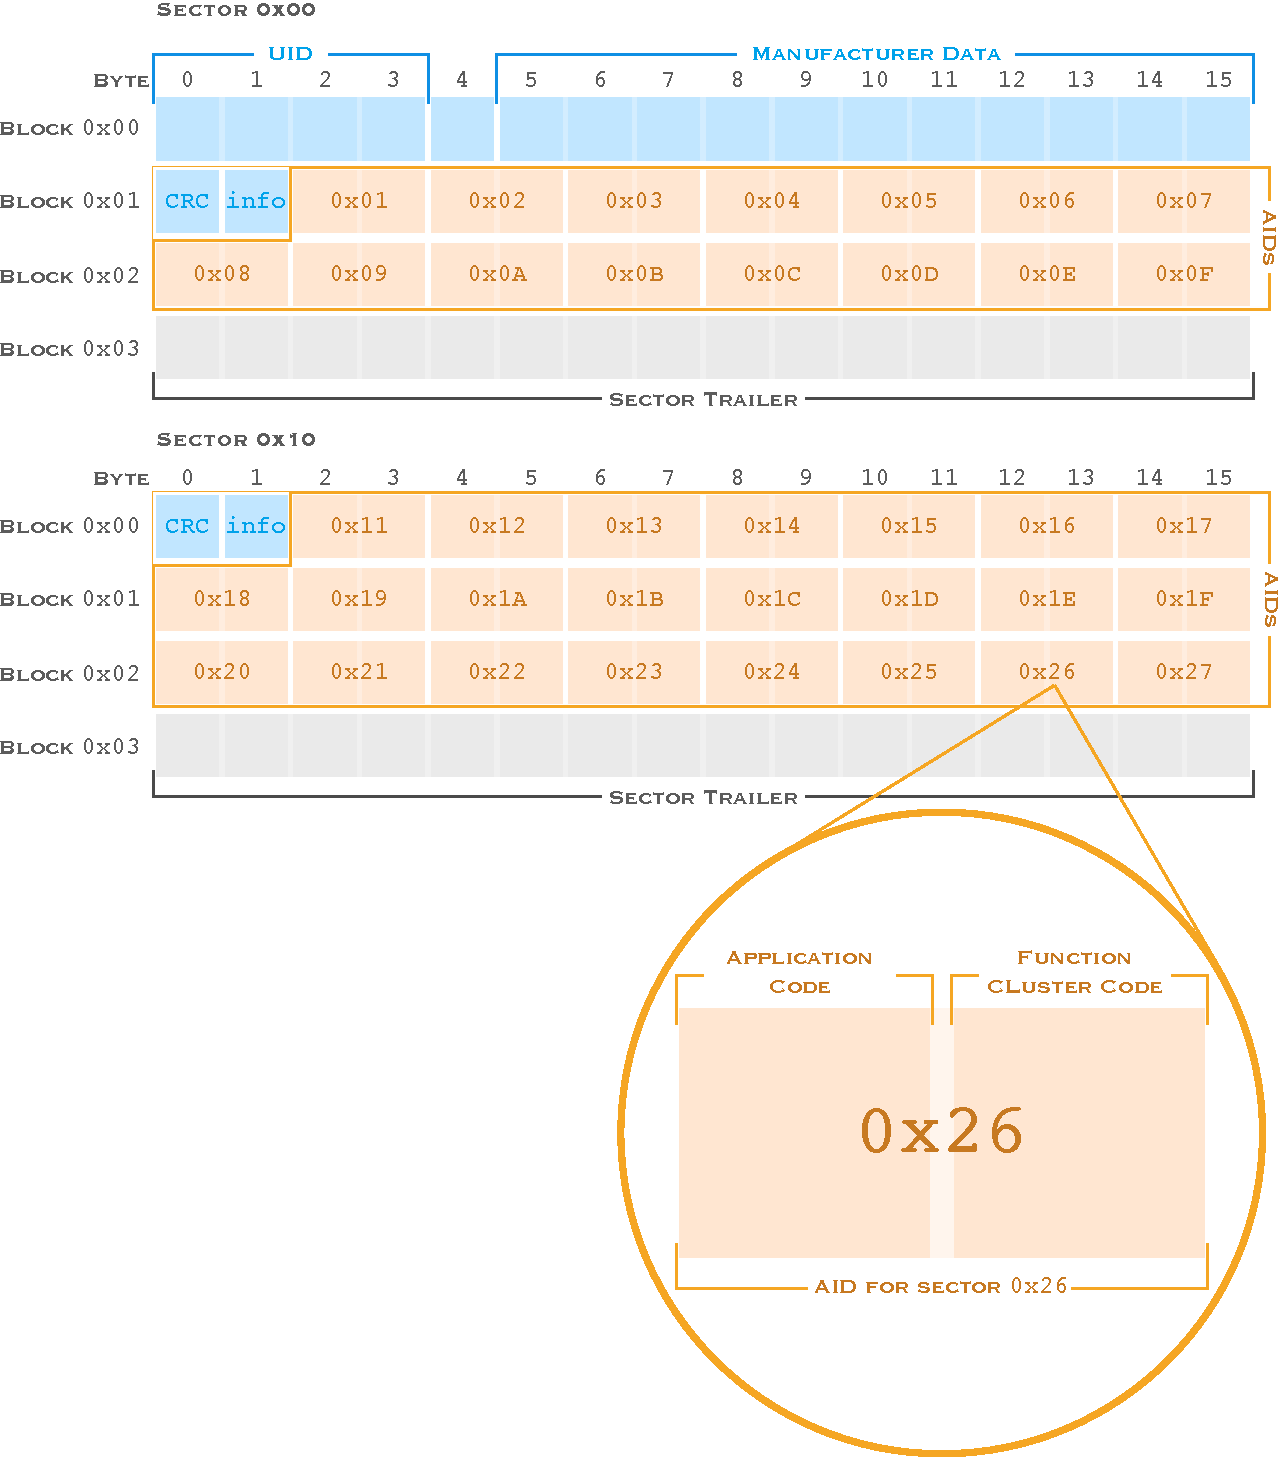
\includegraphics[width=0.8\textwidth]{mad_structure.pdf}
    \caption{Structure of the \mifare{} Application Directory}\label{fig:mad_structure}
  \end{figure}

  The \texttt{MAD} interface has a method for looking up the AID for a sector and for allocating sectors for a new application of a given size.

  \begin{code}[numbers=none]{Go}
    // MAD represents the Mifare Application directory. On 1kB cards
    // the MAD is located in sector 0x00, on 4kB cards it is located in both
    // sectors 0x00 and 0x10.
    //
    // The MAD is essentially a map from sector numbers to the corrresponding
    // application ID.
    type MAD interface {
    	//AIDForSector returns the AID for the corresponding sector
    	AIDForSector(sector byte) AID

    	// AllocApplication allocates enough sectors to store size bytes and then returns
    	// the allocated sectors if successful. If the application has already been allocated
    	// nil is returned.
    	AllocApplication(aid AID, size uint) ([]byte, error)

      // FindApplication returns a slice of sectors that contain the specified application
      FindApplication(aid AID) []byte
    }
  \end{code}


  \subsubsection{Application Identifiers}
  Application IDs are globally registered with NXP, thus preventing two organisations from using the same application ID.\@ The AID consists of two bytes, a one-byte function cluster code and a one-byte application code. The function cluster code determines the classification of application, some examples are:

  \begin{itemize}
    \item \bold{Card Administration} (\texttt{0x00})
    \item \bold{Airlines} (\texttt{0x08})
    \item \bold{Academic Services} (\texttt{0x58})
    \item \bold{Ministry of Defence, Netherlands} (\texttt{0x4A})
    \item \bold{Ski Ticketing} (\texttt{0x50})
  \end{itemize}

  The application code is incremented each time a new AID is registered within a function cluster code.

  The library exports the following interface for an AID:\@
  \begin{code}[numbers=none]{Go}
    // AID represents an Application ID.
    // AIDs consist of a function cluster code and an application code. The former
    // identifies the broad category of the application (e.g. bus services / access
    // control and security) and the latter the specific registration.
    // AIDs must be registered with NXP, a list of current registrations can be found
    // here: http://www.nxp.com/documents/other/MAD_list_of_registrations.pdf
    type AID interface {
    	ApplicationCode() byte
    	FunctionClusterCode() byte
    }
  \end{code}

  Given the simplicity of the AID, the library provides a universal implementation that each driver can use. The implementation is simply a 2-byte array with methods for returning the function cluster code and application code.

  The library has constants for each function cluster code. This makes code that uses the library easier to read as rather than an opaque byte value a descriptive constant name is used.

  The \mifare{} specification defines some reserved AIDs for card administration. These AIDs are also provided.

  \begin{code}[numbers=none]{Go}
    var (
    	// FreeAID is used for sectors that are free
    	FreeAID = NewAID(CardAdministration, 0x00)

    	// DefectAID is used when the sector is defective, e.g. secret keys are
    	// destroyed or unknown
    	DefectAID = NewAID(CardAdministration, 0x01)

    	// ReservedAID is used when the sector is currently free but has been reserved
    	ReservedAID = NewAID(CardAdministration, 0x02)

    	// AdditionalDirectoryInfoAID is useful for future cards where the directory
    	// needs more sectors
    	AdditionalDirectoryInfoAID = NewAID(CardAdministration, 0x03)

    	// CardHolderInfoAID is used for a sector that contains card holder info in
    	// ASCII format
    	CardHolderInfoAID = NewAID(CardAdministration, 0x04)

    	// NotApplicableAID is used when this sector doesn't exist on the card
    	NotApplicableAID = NewAID(CardAdministration, 0x05)
    )
  \end{code}

  \subsection{Drivers}
  The library contains two drivers, one which sits on top of \texttt{libnfc} and interacts with physical cards and a mock driver which is used for testing and simulation. Because of the way the library is structured a third party could implement their own driver, provided it satisfies the above interfaces.

  \subsubsection{Libnfc Driver}
  The libnfc driver doesn't interact with \texttt{libnfc} directly. As shown in Figure~\vref{fig:lib_structure}, the driver sits on top of a ``thin binding''\footnote{A thin binding allows code in one language to call functions from a library written in another. A thick binding provides its own API that sits on top of the library, making the exposed API more idiomatic to the new language.} that allows it to call C functions from within Go. This binding sits on top of \texttt{libfreefare}, the part of \texttt{libnfc} which has support for \mifare{} cards.

  \begin{figure}[h]
    \centering
    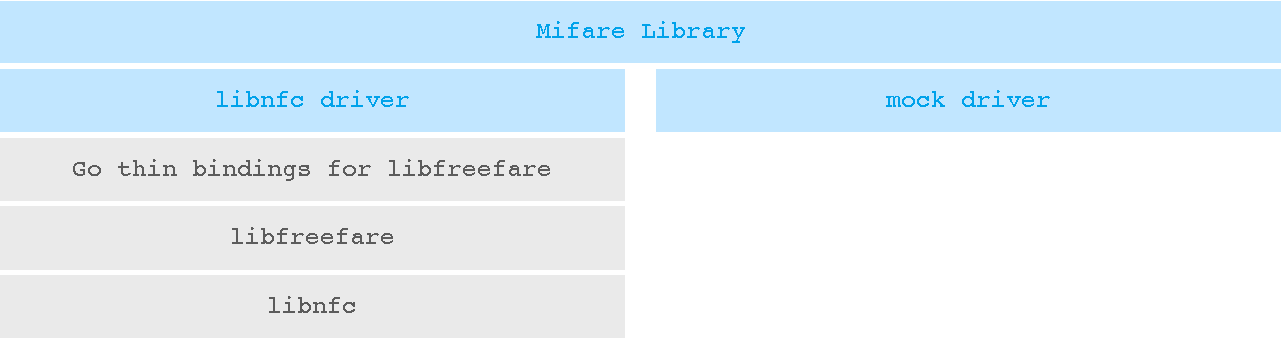
\includegraphics[width=0.8\textwidth]{library_structure.pdf}
    \caption{Structure of the \mifare{} Library}\label{fig:lib_structure}
  \end{figure}


  \subsubsection{Mock Driver}

  The mock driver provides a software implementation of the \mifare{} Classic card. This is useful for both testing and simulation. The scope of the mock driver is sufficiently larger than that of the \texttt{libnfc} driver due to the necessity of implementing all of the card logic in software.

  \bold{Structure of Mock Card} \\
  As shown below, the mock card is a struct containing a field specifying whether it is a 1K or a 4K card and an array of blocks.

  \begin{code}[numbers=none]{Go}
    type classicTagImpl struct {
    	tagType mifare.TagType
    	blocks  [256][16]byte
    }
  \end{code}

  \bold{Access Bits} \\
  The access bits in the sector trailer control which memory operations are permitted by each key. There are 12 access bits, each access bit is stored once non-inverted and once inverted as shown in figure~\vref{fig:access_bits_structure}. Whenever an operation is performed, the format of the access bits is verified and if a violation is detected the sector is irreversibly blocked, thus preventing corruption of a single bit from allowing unintended access.

  \begin{figure}[h]
    \centering
    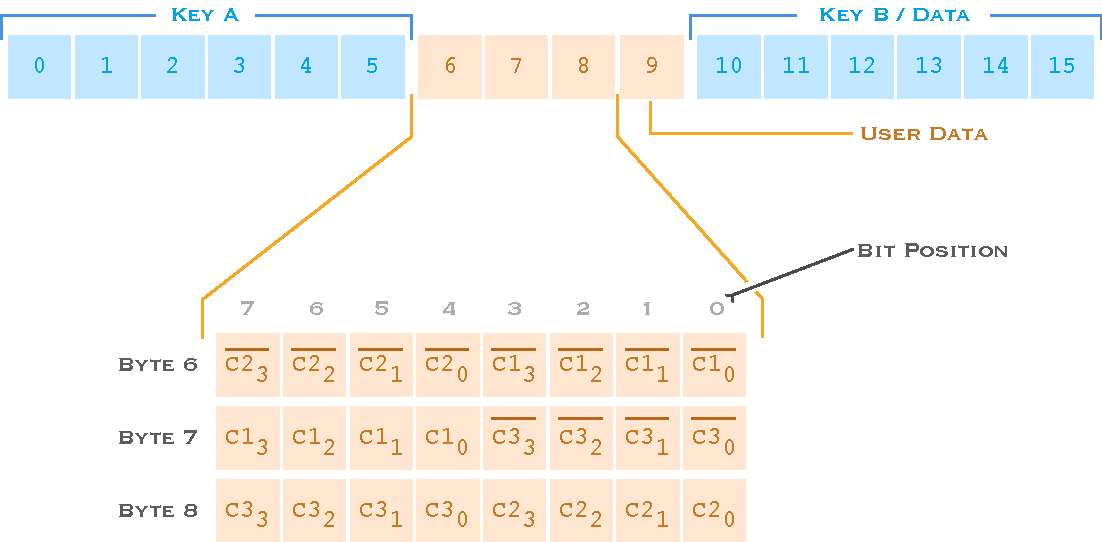
\includegraphics[width=0.9\textwidth]{access_bits_structure.pdf}
    \caption{Access Bits Layout}\label{fig:access_bits_structure}
  \end{figure}

  The access bits are split into four sets of three bits (in figure~\vref{fig:access_bits_structure} $C2_0$ denotes the second bit of the first set). Each block in the four-block sectors including the sector trailer has its own set of three access bits and thus each block can have different access conditions. For 16-block sectors the 4 sets of access bits are divided between the blocks such that one set of access bits ($C1_3 C2_3 C3_3$) still controls access to the sector trailer and each of the remaining three sets of access bits controls access to five contiguous blocks as shown in figure~\vref{fig:access_bits_sector}.

  \begin{figure}[h]
    \centering
    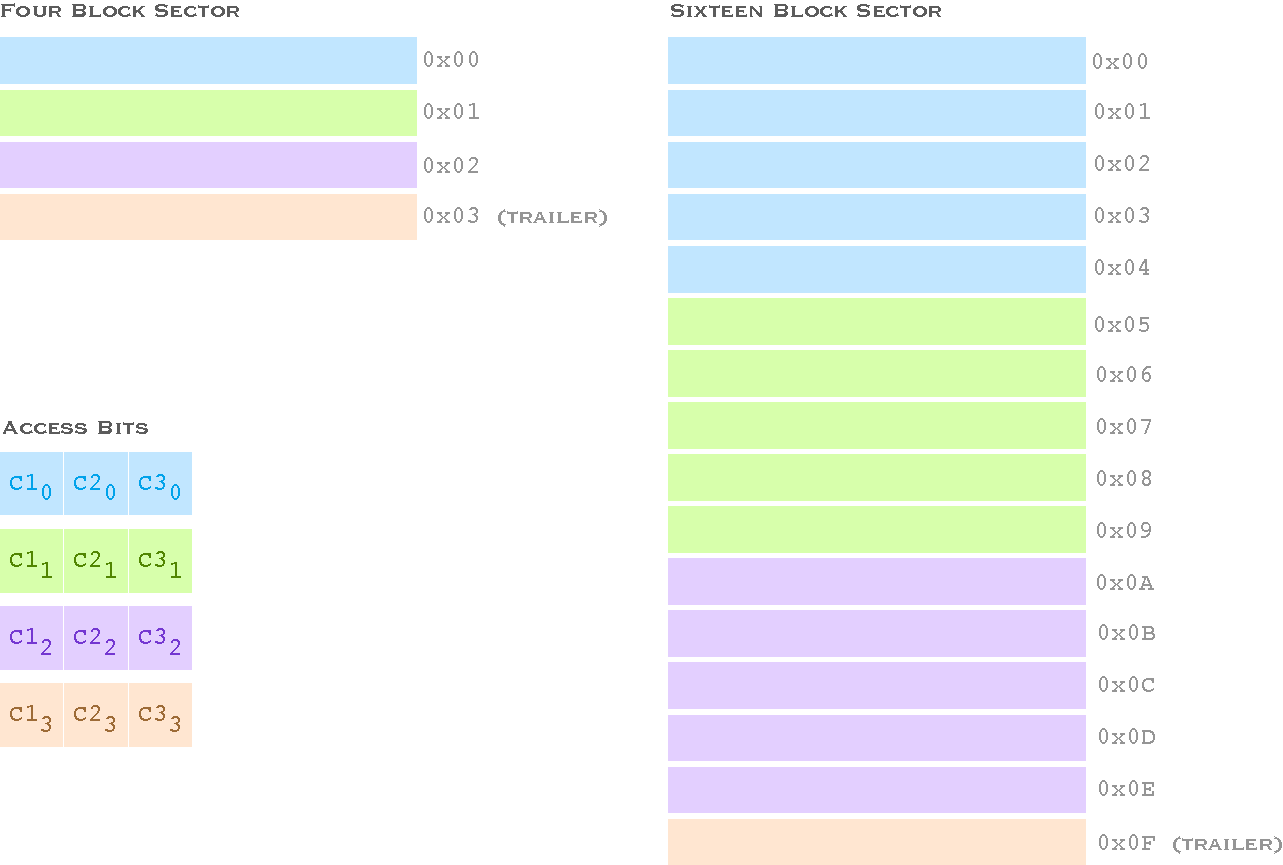
\includegraphics[width=0.8\textwidth]{access_bits_sector.pdf}
    \caption{Block Division for Access Conditions}\label{fig:access_bits_sector}
  \end{figure}


  \section{Digital Signature Protection}
  Recall from Section~\vref{sec:mad} that the \mifare{} Application Directory is a lookup table stored in sectors \texttt{0x00} and \texttt{0x10}. For each sector on the card, the MAD stores the application ID (AID) corresponding to the data in that sector. By registering an AID for digital signatures and using the MAD the signature can be placed anywhere on the card where there is sufficient available space. By not relying on a static sector number the scheme can remain agnostic of the existing data layout.

  \subsubsection{Signature Structure}

  The signature consists of a 16-byte header followed by the raw signature bytes. The header contains the following as shown in figure~\vref{fig:signature_structure}.

  \begin{itemize}
    \item \bold{Signature Scheme Version} (\SI{1}{byte} in sector trailer) \\
      To allow for backwards incompatible changes to the scheme a \SI{1}{byte} version number is included. This is set to \texttt{0x01} for this version of the scheme. Without this, any backwards incompatible changes would require a new signature AID.\@ The byte is stored in the sector trailer.

    \item \bold{Key Identifier (KID)} (\SI{2}{bytes}) \\
     The KID is an opaque identifier that the organisation increments every time they use a different key or signing algorithm. This KID allows a reader to be able to determine which key and signing algorithm was used to create a signature and therefore provides support for changing the signing key or algorithm.


    \item \bold{AIDs} (\SI{14}{bytes}) \\
      The last \SI{14}{bytes} of the header specifies the data that is signed, it consists of a sequence of \SI{2}{byte} values. Each \SI{2}{byte} value is the AID of an application that is signed. Within this context the ``not applicable'' AID (\texttt{0x0005}) is repurposed to mean the card UID.\@
  \end{itemize}

  \begin{figure}[h]
    \centering
    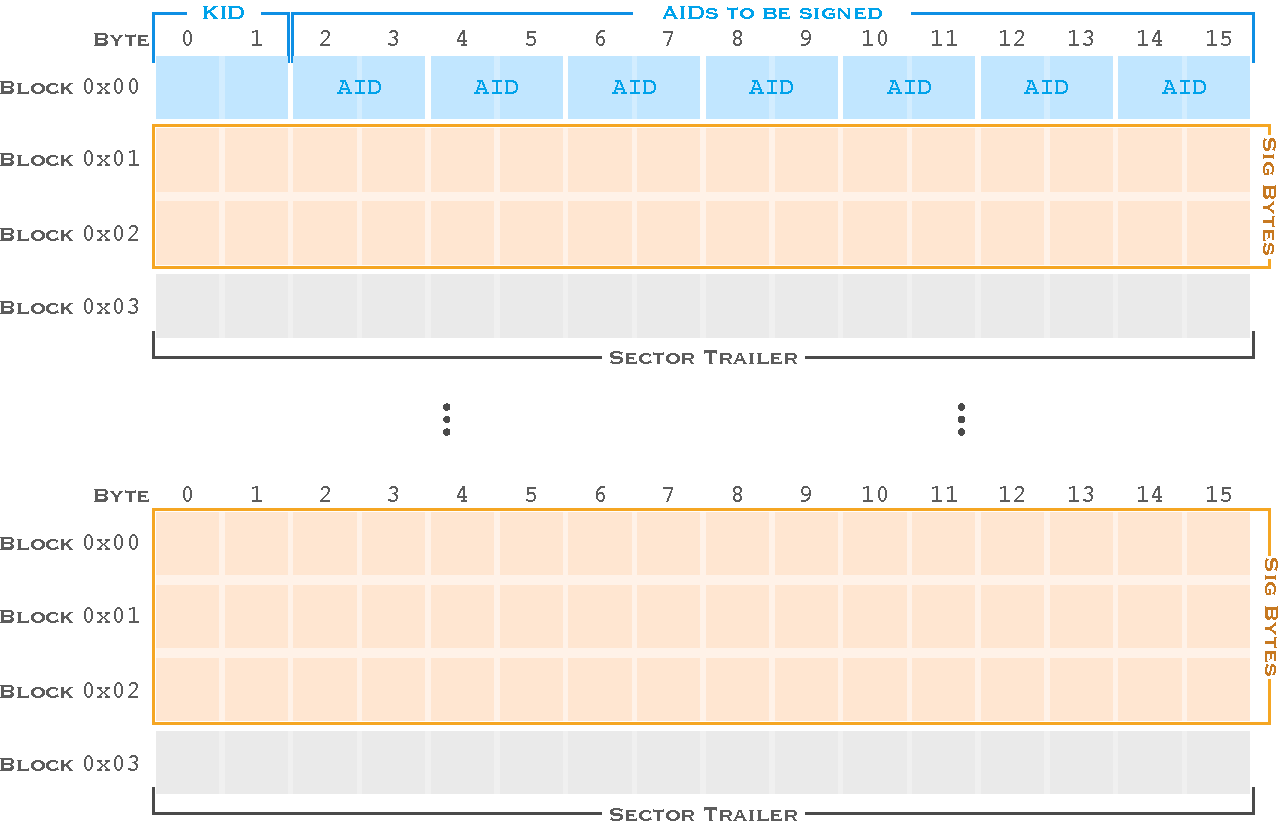
\includegraphics[width=0.9\textwidth]{signature.pdf}
    \caption{Signature Structure}\label{fig:signature_structure}
  \end{figure}

  The structure and length of the signature bytes section depends on the signing algorithm used. The scheme is agnostic of this, the KID specifies which key and signing algorithm was used. This allows third parties to implement their own signing algorithms if they are not satisfied by the implementation provided.

  \subsubsection{Signature Scheme}
  The signature scheme specifies which data and in what order it is passed to the signing algorithm. The data to be signed consists of the following:
  \begin{enumerate}
    \item \bold{The signature header}
    \item \bold{7 bytes for the application lengths} \\
      For each AID in the signature header, a byte is included specifying the number of blocks of data for that application. If the AID is \texttt{0x0000} then \texttt{0x00} is the byte value used.
    \item \bold{The application bytes} \\
      For each AID in the signature header, the application data is added. If the value corresponds to the ``not applicable'' AID then the UID is added. If the AID is \texttt{0x0000} then no data is added.
  \end{enumerate}

  Pseudo code of the signature algorithm is included below.
  \begin{code}[numbers=none]{python}
    payload = []
    payload.append(header.kid)

    for aid in header.aids:
        payload.append(aid)

        if aid == 0x0000:
            payload.append(0)
        else if aid == NotApplicableAID:
            payload.append(len(uid))
            payload.append(uid)
        else:
            payload.append(num_blocks(aid))
            payload.append(get_data(aid))

    def get_length(aid):
        if aid == 0x0000:
            return 0
        if aid == NotApplicableAID:
            return len(uid)
  \end{code}

  \subsection{Digital Signature Library}
  The digital signature library is written in Go and sits on top of my \mifare{} library. The implementation provides the following:

  \begin{itemize}
    \item \bold{Elliptic Curve Keypair Generation Program} \\
      The library contains a method and command line interface for creating new elliptic curve key-pairs.

    \item \bold{Method for Allocating Signature} \\
      This method is used to provision a new signature. It does the following:
      \begin{itemize}
        \item Allocate sectors for the signature by writing to the application directory.
        \item Update the sector trailers with the new keys.
        \item Write the signature header.
      \end{itemize}
    \item \bold{Method for Writing Signed Data} \\
      This method wraps the \texttt{WriteApplication} method from the \mifare{} Library and additionally updates the signature.

    \item \bold{Method for Reading Signed Data} \\
      This method wraps the \texttt{ReadApplication} method from the \mifare{} Library and checks that the signature is present and valid.
  \end{itemize}

  \subsubsection{Signing Algorithm}
  As previously mentioned, the scheme does not dictate which signing algorithm to use. However, for the library to be plug-and-play it would have to contain at least one signing algorithm implementation. I chose to implement the elliptic curve digital signature algorithm (ECDSA) as it produces much smaller signatures for the same level of security as its RSA equivalent. Keeping the memory footprint of the signatures as small as possible is desirable given the memory constraints of the card.

  \subsubsection{Elliptic Curve}
  An elliptic curve has to be chosen before creating an elliptic curve private key. The National Institute of Standards and Technology has standardised several curves including \texttt{P-224}, \texttt{P-256} and \texttt{P-384}. Each curve has slightly different properties.

  There is a suspicion amongst some security researchers that the NIST standardised elliptic curves may have been backdoored by the NSA.\@ Each curve contains an unexplained seed value from which coefficients are generated. The suspicion is that these seed values could have been created in such a way as to weaken the security of the curves they produce in an as-of-yet unknown way. This property is called elasticity.

  As of Go 1.6, the standard library only has support for these NIST curves. There are some independently maintained implementations of other curves but the authors stress that they haven't been peer reviewed and shouldn't be used where security is paramount. Because of how the digital signature library is structured it will support additional curves without modification when they are introduced into the standard library.

  \subsubsection{Unit Tests}

  The digital signature library contains a comprehensive test suite. By using the \mifare{} library it has been possible to write unit tests that do not depend on a physical card.

  \subsection{Difficulties Overcome}
  \subsubsection{AID Swap Attack}
  % attack
  During development of the digital signature library I discovered a vulnerability in my original proposal that would allow an adversary to manipulate the data whilst retaining a valid signature in certain circumstances.

  To illustrate the attack, suppose that a card has two applications on it, $A$ and $B$ that are stored in sectors $1$ and $2$ respectively. The signature header specifies that the signature is across applications $A$ and $B$ and thus sectors $1$ and $2$, in that order.

  Now suppose an adversary swaps the order of the applications in the signature header, and changes the application directory such that $A$ now points to sector $2$ and $B$ points to sector $1$. The signature is now across $B$ and $A$ (wrong way around), however this still resolves to sectors $1$ and $2$ (right way around) and thus the signature is still valid. If a reader attempts to read application $A$ it will get the data for application $B$ and vice versa.

  To mitigate this, I altered the implementation such that the signature header is always included in the data that is signed, thus preventing an attacker from tampering with it.

  \subsubsection{Application Length Malleability Attack}

  Suppose that a card has two applications on it, $A$ and $B$. $A$ is stored in sectors $1$ and $2$ and $B$ is stored in sector $3$. If an attacker changes the application directory such that $A$ points to sector $1$ and $B$ points to sectors $2$ and $3$ then the signature would still be valid.

  To mitigate this attack I added the application length to the signature payload.

  \section{Revocation Simulation Suite}

  The simulation suite models a network of readers and simulates cards traveling through the network. It records how many cards travelled through each reader before a revoked UID was propagated to it.

  \subsection{Reader Network Topology}\label{sec:topology}
  The network of readers is represented as a directed graph. Nodes represent readers and the directed edges from one node lead to all the readers that can be accessed after going through that reader. The indegree of a reader is the number of readers from which someone at this reader could have come from.

  The simulation suite contains a generator that returns a semi-randomised topology based upon the number of offline and online readers. The indegree of each reader (the number of readers that it is accessible from) is assigned randomly from the range $1$ to $\sqrt{{num\_readers}}$. The edges for each reader are then assigned randomly to satisfy the indegree. After this, a sanity check ensures that every reader has an edge to another one, if a reader doesn't then a new edge is added. This ensures that the simulation doesn't get stuck.

  \subsection{Card Simulation}
  The simulation is based on discrete time-steps. At each time-step every card moves to a new reader by choosing an available edge at random. The definition of a time-step is left intentionally vague, as any meaningful comparison with actual time is very much dependent on the frequency with which cards are used in the network. Some deployments will have cards that typically tap a dozen readers a day and others will have cards that stay dormant for months.

  \section{Revocation Gossip Protocol}

  The gossip protocol\footnote{A gossip protocol is a type of computer-to-computer communication protocol that disseminates information throughout a network in a manner much like how rumours are spread throughout an office.} enables the distribution of revoked card UIDs to offline readers by using the spare space on the cards. The development of the revocation gossip protocol was iterative. At each stage of development, the simulation suite identified specific areas of weakness, thus informing further iterations. Given the explorative nature of development, this section outlines each implementation in detail rather than the one which performed best. This helps to give context and justify the motivating factors behind each change made.

  \subsubsection{Na\"{\i}ve Implementation}
  The na\"{\i}ve implementation involves online readers storing a list of the revoked UIDs on the card. When the card is tapped on an offline reader the reader updates its internal list of revoked UIDs. When the number of revoked UIDs exceeds the number that can be stored on the card the most recently revoked ones are used.

  This implementation is clearly not perfect, the revocation sector on the card has a restricted amount of storage. If more cards are revoked at one time than can be stored in the revocation sector, this implementation will fail to distribute some of them. The implementation is useful for assessing the performance of others. When the rate at which cards are revoked is sufficiently low the na\"{\i}ve approach is close to being optimal and thus provides a convenient baseline to indicate the inherent difficulty of a particular simulation configuration.

  \subsubsection{Random Implementation}
  Each time a card is tapped on an online reader this implementation chooses a random subset of the revoked card UIDs to place on the card.

  The random implementation performs very well when the total number of revoked cards is low, however as can be seen from Figure~\ref{fig:chain_1000_impl}, as the number of revoked cards increases, the performance decreases. This is because the probability that any given UID will be placed on a card is inversely proportional to the total number of revoked cards. As the total number of revoked cards increases, each new revoked UID is placed onto fewer cards with an increasing amount of the storage on each card being used for UIDs that have already been propagated throughout the network.

  \begin{figure}
  \centering
  \begin{subfigure}{.5\textwidth}
    \centering
    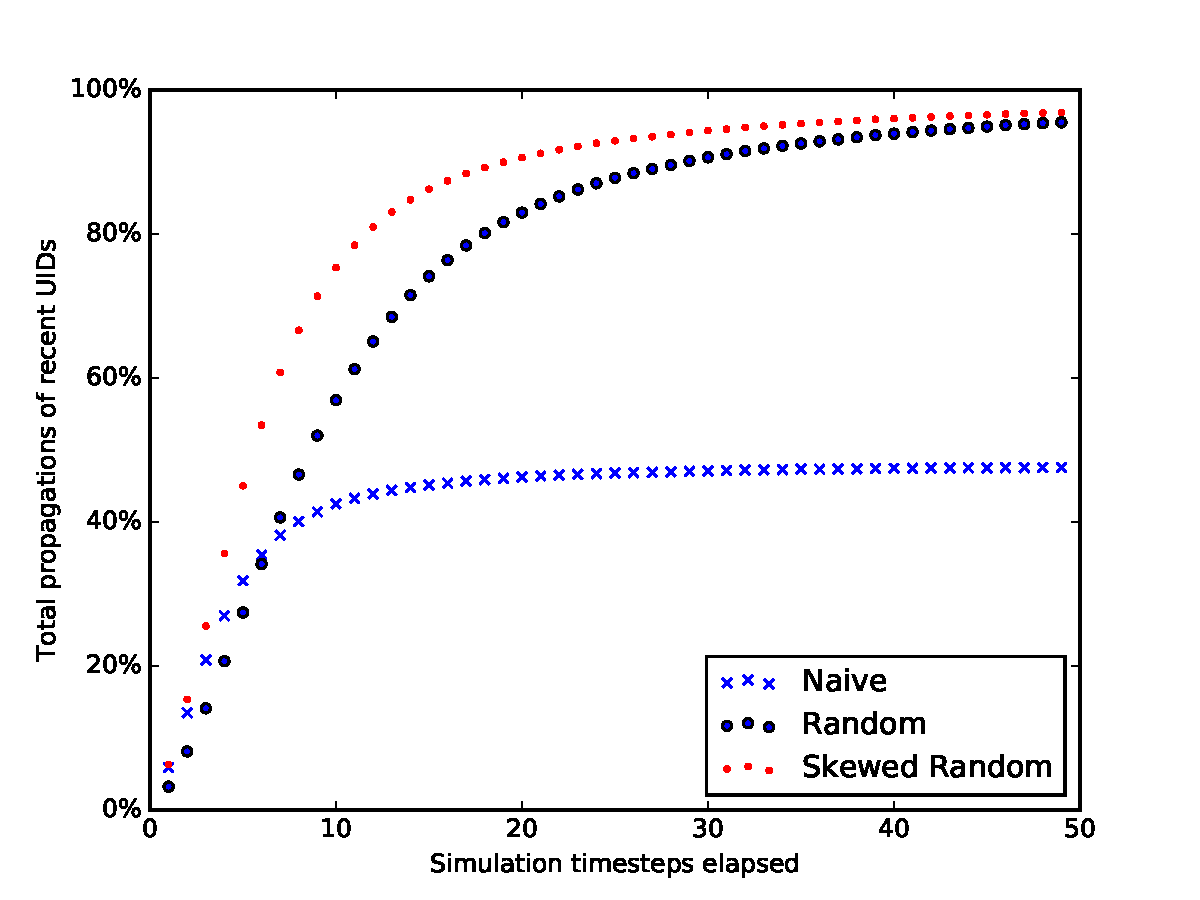
\includegraphics[width=\linewidth]{chain_1000_25_25.pdf}
    \caption{Performance with 25 existing UIDs}
  \end{subfigure}%
  \begin{subfigure}{.5\textwidth}
    \centering
    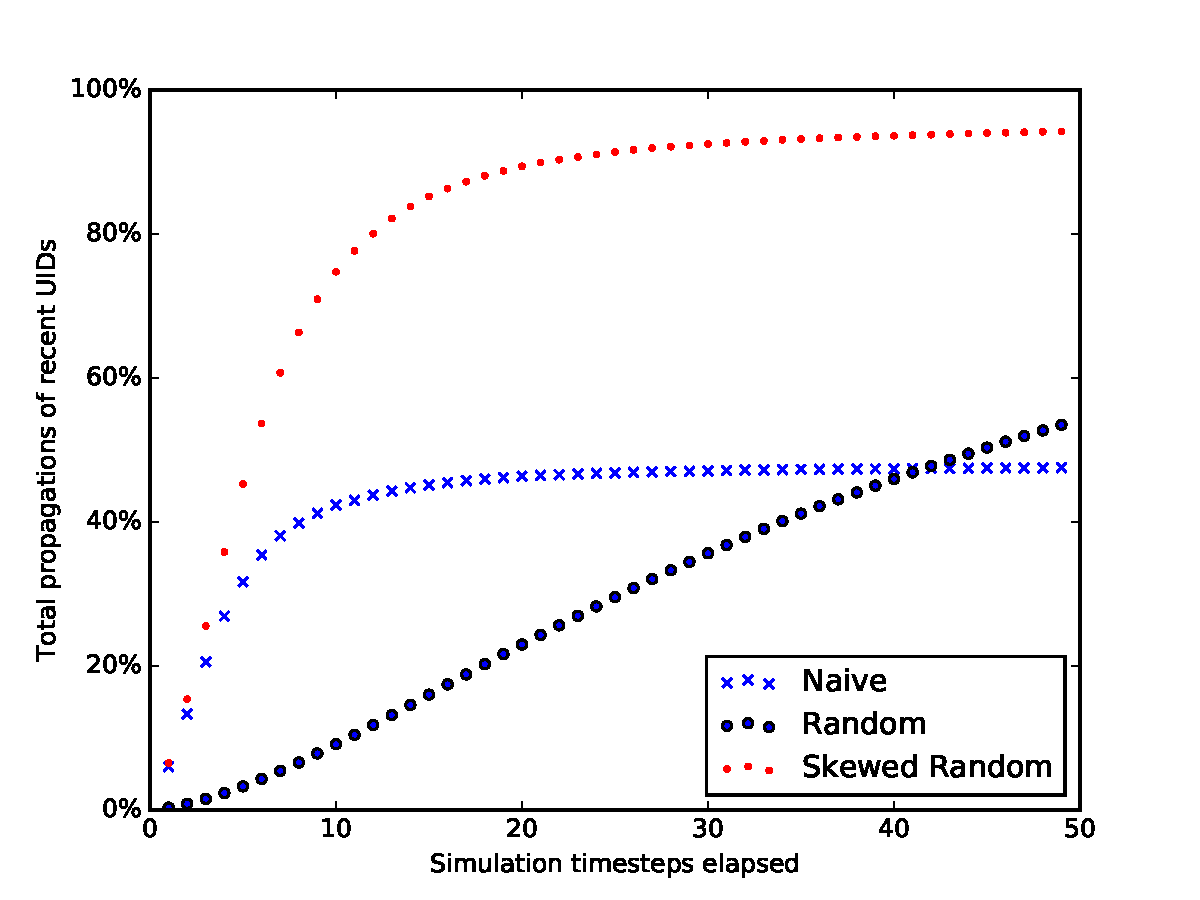
\includegraphics[width=\linewidth]{chain_1000_500_25.pdf}
    \caption{Performance with 500 existing UIDs}
  \end{subfigure}%
  \caption{Performance with varying numbers of fully propagated UIDs}\label{fig:chain_1000_impl}
  \end{figure}


  \subsubsection{Skewed Random Implementation}\label{sec:skewed}

  The random implementation performed well initially but the simulation suite demonstrated that as the total number of revoked cards grew, its performance suffered. To improve its performance with a large number of revoked cards it is necessary to ensure that the probability of a recently revoked UID being placed on a card is independent of the total number of revoked cards.

  The skewed implementation does this by prioritising UIDs that have not been placed onto 5 cards. Each online reader maintains two buckets (arrays) of UIDs and a count of how many times each UID has been distributed. When a UID has been distributed 5 times, it is moved from the first bucket to the second. UIDs in the first bucket are always chosen before those in the second.

\end{document}
